\chapter{Critère de choix d'une tentacule}
\begin{figure}[!ht]
    \centering
    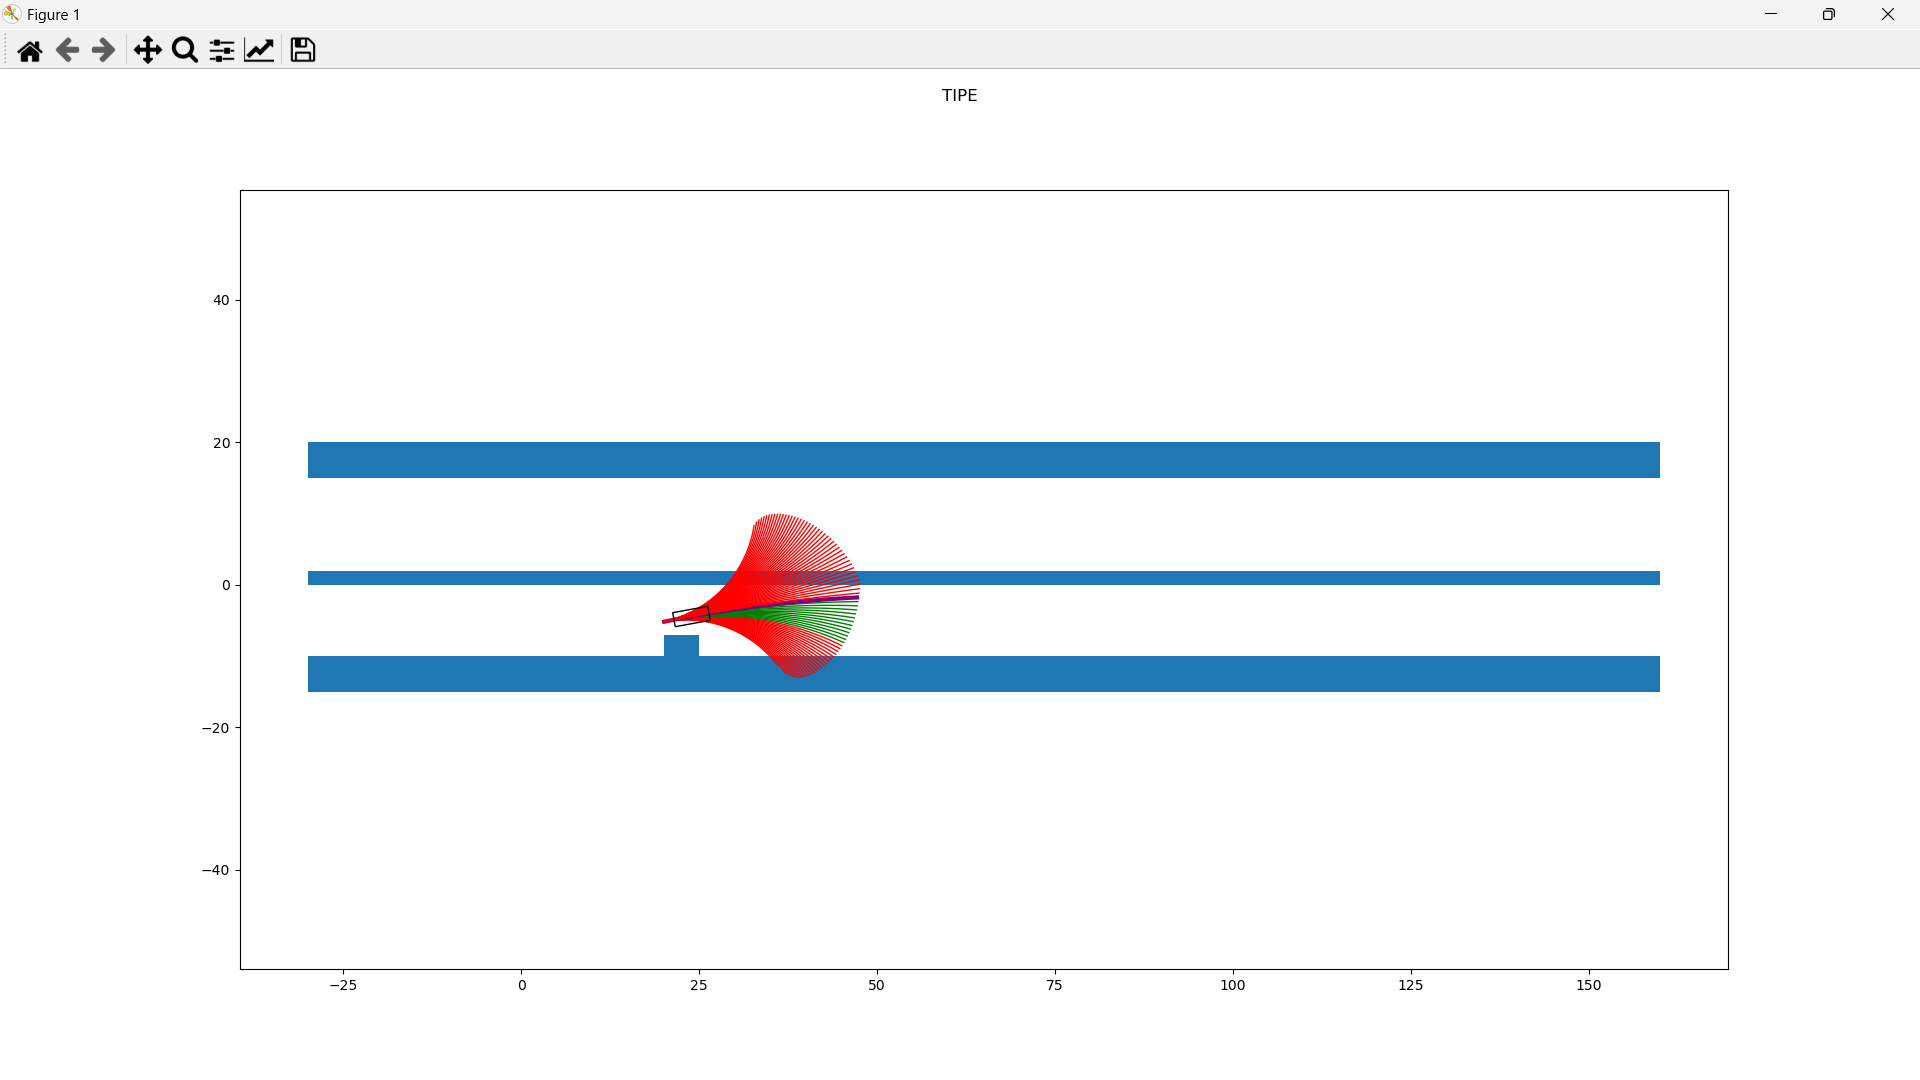
\includegraphics[scale=0.4]{evitement simple.png}
\end{figure}
\vspace{100pt}

\begin{mintedbox}{python}
"""
Déplace la voiture de manière optimal sur un parcours.
"""
class Tentacule:
    """
    Objet tentacule, dépendant d'une voiture, et déterminé par son ordre et son angle de braquage.
    """

    def __init__(self, voiture, k, delta_k, axes):
        self.V_lisse = abs(self.braquage - self.voiture.braquage) / (2 * self.voiture.braquage_max)


class Voiture:
    """
    Objet voiture, défini par sa forme. D'autres paramètres fixes sont définis après, on pourra les mettre en paramètre plus tard si plusieurs voitures il y a.
    """
    def choix_tentacule(self, tentacules_navigables):
        # TODO : faire un critère de dégagement du tentacule (p. 125 section 9.2.4.1)
        # TODO moins important car nécessite GPS et tt (pas forcément notre objet d'étude) : faire un critère de rapprochement de la trajectoire globale (p.126 section 9.2.4.3)

        try:
            return min(tentacules_navigables, key=lambda x: x.V_lisse**4 + x.braquage**2)  # On trie selon une loi fonction de V_lisse (écart au braquage actuel) et de braquage (trajectoire droite). Puis on prend le min
        except ValueError:
            print("AUCUNE TENTACULE NAVIGABLE")

\end{mintedbox}
